% !TeX root = ../thesis.tex
\subsection{Machine learning}
\label{lr_sec:machine_learning}
\paragraph{}
A machine learning algorithm is such an algorithm that is able to learn from data and find regularities.
The ``learning'' is defined as ``A computer program is said to learn from Experience E with respect to some class of tasks T and performance measure P, if its performance at tasks in T, as measured by P, improves with experience E.'' \citep{Mitchell:1997:ML:541177}
\paragraph{}
The tasks T refer to the task that are too hard to solve with fixed programs.
For example, if a robot is designed to be able to walk, it can be done by a program that help the robot to learn how to walk or by a program written manually to tell the robot how to walk.
The second option is rarely chosen because a fixed program can hardly adapt the complex situation in the reality.
The tasks usually include classification and regression problems in numerical calculation.
% The task in adaptive analysis will be classification.
% In this type of task, the algorithm is required to specify which category some input belongs to.
% Solving this task is to find a function $f: \mathbb{R}^n \rightarrow \{0,1\}$ where $0$ stands for ``not refine'' and $1$ for ``refine''.
% Each variable in the vector of the input $\pmb{x}$ in the function $y=f(\pmb{x})$ is a feature.

\paragraph{}
As a way to measure the abilities of a machine learning program, quantitative measurement of its performance must be designed.
Accuracy could be one of the most popular performance measurement in classification task.
It is simply defined as the rate of examples for which the algorithms gives the same classification as the reality.
In real world problem, the ability that a model performs on data that it has not seen before could be more important as it is related to its performance when used in real world problem\hl{s}.
Consequently, these performance measures are usually evaluated using a subset of the original data called test set.
While another subset of the original data called training set is adopted to train the machine learning system.

\paragraph{}
A learning algorithm normally is either unsupervised learning or supervised learning.
It is dependent on what kind of experience it has during the learning process.
Unsupervised learning algorithms experience a dataset that have a series of features.
It is expected to learn useful properties of this dataset.
While supervised learning algorithms experience a dataset that not only have many features, but also have a label or target.
For example, in Iris Fisher data set \citep{Fisher1936}, fish species of each iris plant will be included as well as features of the fish. 

\paragraph{}
The machine learning algorithms targeting classification problems used in the proposed method will be introduced in Sec.~\ref{lr_sec:MLP}.

% ------------------------------------------------------------------------------------ %
\subsection{Multilayer perceptron(MLP)}
\label{lr_sec:MLP}
\paragraph{}
There are plenty of machine learning algorithms such as Support Vector Machine (SVM) \citep{Boser1996,Cortes1995}, decision tree \citep{Olshen1984}, random forest \citep{Ho1995}, etc. that can be adopted in all kinds of situation.
Multilayer Perceptron (MLP), also known as feedforward neural networks or deep feedforward networks will be introduced in detail in this section.

\paragraph{}
Fig.~\ref{lr_fig:ml_mlp_intro} illustrates a typical multilayer perceptron.
The reason why it is called feedforward is because that all calculation are conducted all the way from the inputs $x$ to the outputs $y$, passing the intermediate computations.
There is no feedback from a deeper layer to a shallower layer otherwise it becomes a recurrent neural network.
It is called neural networks is because that they are usually defined by a composition of several distinct functions.
These functions can be described as an acyclic graph.
Take a function $f(x) = f^{(3)}(f^{(2)}(f^{(1)}(x)))$ as an example, it describes a MLP with three layers.
In this example, $x$ will be the input and the function $f^{(1)}$ is the first layer, $f^{(2)}$ being the second and the $f^{(3)}$ is called the output layer.
Number of the functions or the length of the chains is called the depth of the neural network.
When a neural network with large number of layers, it is consider as a deep neural network and it is where the term ``deep learning'' comes from.
The training purpose of a MLP is to predict the output $y_p$ that is close to the accurate value $y_a$ from any given input $x_p$.
A training set with both inputs $x_t$ and expected outputs $y_t$ specify directly the behavior of the output layer upon different inputs.
There is no direct relationship between what other layers do and the training data.
A suitable learning algorithm is expected to be able to train these intermediate layers to response properly so that the prediction from the output layers is accurate enough.
These intermediate layers are called hidden layers as they are not directly related to the desired outputs.
\paragraph{}
Furthermore, the word neural illustrates that the idea of the topological model comes from neuroscience.
In the mathematical model of the neural network, each unit in a layer acts independently like a neuron in human being's brain.
Even though a layer of these `neurons' forms a vector, the model can be more suitably described by each layer contains some neuron that behave analogously (dot production between two vectors) instead of a layer to layer relationship (matrix production between a vector and a matrix).
The choice of selecting more than one layers of vector and each neuron takes all values from the previous layer and then computed its own value to describe the model comes from the neuroscience while the functions used in the model are not guided by the neuroscience but by mathematical and engineering technologies.
A neural network so far will never aim to simulate a brain perfectly as well, it is designed to achieve statistical generalization instead.

\begin{figure}[!ht]
    \centering
    \scalebox{0.3}{
        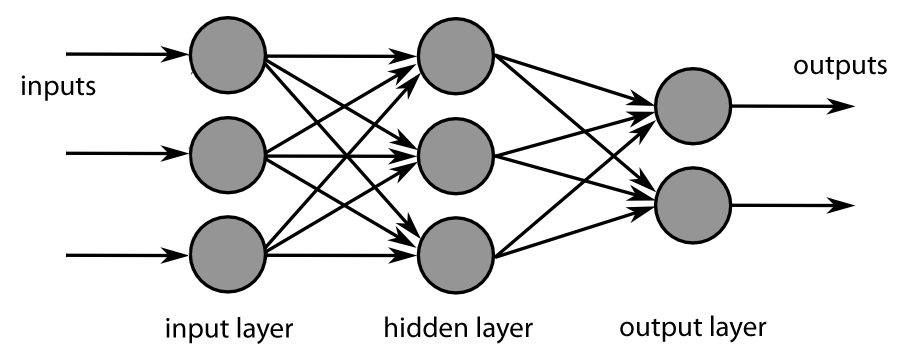
\includegraphics{literature/images/mlp_intro.png}
    }
    \caption[A typical topology of a multilayer preceptron]{A typical topology of a multilayer preceptron}
    \label{lr_fig:ml_mlp_intro}
\end{figure}
%
The key question of a MLP is how to find a proper non-linear mapping function $\phi_i$ that can calculate all units in $i+1$-th layer from the previous one.
One of the options is to adopt a generic function, such as the Radial Basis Function(RBF)\citep{chang2010} kernel.
Even though an RBF kernel is capable to fit the training data with infinite-dimensional function, the performance on the test set usually not as satisfactory as it is on the training set.
Some advanced example can not be solved as not enough prior information is encoded and generic feature mappings drawn from the local smoothness is used only.
Another widely-accepted approach before the concept of deep learning being popular is to set the function manually.
Each used function for separated task typically spends engineers decades of time and it is very unlikely that these functions can be used in other fields.
The strategy of deep learning is to find the function by itself based on the given training set.
In this approach, we have a model $y=f(x;\theta,\omega)=\phi(x;\theta)^T\omega$.
Where $\theta$ stands for parameters used to learn function $\phi$ from a large variety of functions.
Parameters $\omega$ then map the intermediate result $\phi(x)$ to the desired output.
Drawback of this method is that the convexity will not be guaranteed during the searching of the global minimum which means finding a local minimum based on gradient no longer gives a global minimum.
However, the merits outweigh the shortcomings since the generalization is as high as using an RBF kernel and no human efforts is required.

\subsection{Gradient based optimization}
\paragraph{}
The learning problem of the MLP can be generalized as a optimization problem in mathematics.
In other words, the learning algorithm is to find the global minimum of a specific value on a high dimensional surface.
The function need to be minimized is called the criterion and it is called cost function or loss function when it is being minimized.
Fig.~\ref{lr_fig:ml_gradient_optimization} illustrates how the derivatives are used to perform a gradient descent algorithm on a parabola.
\begin{figure}
    \centering
    \scalebox{0.75}{
        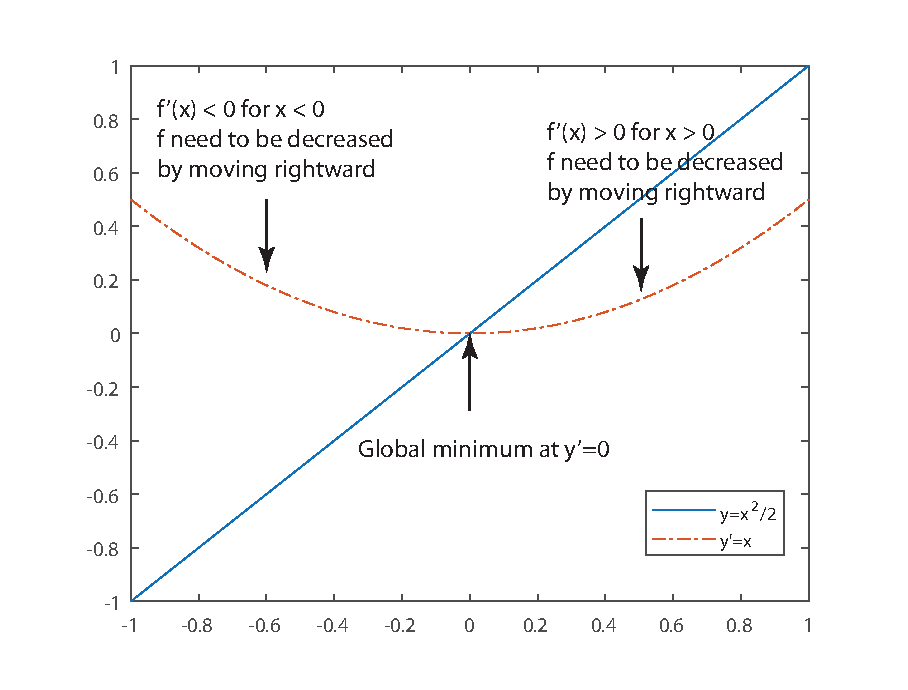
\includegraphics{literature/images/gradient_optimization.eps}
    }
    \caption[Example of gradient descent algorithm on a parabola]{An example of gradient descent algorithm on a parabola}
    \label{lr_fig:ml_gradient_optimization}
\end{figure}
%
In a two dimensional curve which can be expressed by function $y=f(x)$ with real numbers $x$ and $y$.
The derivative $f^\prime=\frac{dy}{dx}$ is ultra useful to determine the global minimal value of a function as it stands for the slope and the slope tells whether $y$ is becoming smaller or larger when $x$ increase.
The global minimal is proven to happen when the derivative equal to zeros or on the boundary if the function is continuous.
While a point with zero slope does not necessary stand for a global minimal as it can be a local one or a saddle point.
\paragraph{}
In training problem\hl{s} of the MLP, chances are that we are end up with a multidimensional function that is not convex which creates extra challenge to determine the global minimal from local ones and saddle points surrounded by very flat regions.
As a consequence, in practice, the algorithm will be terminated when a small enough local minimal is found instead of looking for the global one.
In the situation where multiple inputs are involved, the concept of partial derivatives $\frac{\partial}{\partial x_i}f(x)$ is used to demonstrate the change in $y$ corresponding to the change in the $i$-th input $x_i$.
The gradient $\nabla_x f(x)$ contains the partial derivatives in all directions and hence is used in solving the learning problem in MLP.
In order to minimize loss function $f$, it is expected to determine the direction where $f$ decreases the fastest and it can be expressed in mathematical as \footnote{$\argmin_x f(x) = \left\{
    x | x \in S \wedge \forall y \in S : f(y) \geq f(x)
\right\}$}
\begin{equation}
    \begin{aligned}
    & \argmin_{\mathbf{u}} \mathbf{u}^T \nabla_x f(x)\\
    = & \argmin_{\mathbf{u}} || \mathbf{u} ||_2 ||\nabla_xf(x)||_2 \cos\theta \\
    = & \argmin_{\mathbf{u}} \cos\theta
    \end{aligned}
\end{equation}
%
where $\mathbf{u}$ is a directional unit vector ($\mathbf{u}^T\mathbf{u}=1$) and $\theta$ is the angle between $\mathbf{u}$ and the gradient.
It can be concluded that $f$ can be decreased in the fastest way in the direction of the reverse of the gradient which is called gradient descent in Eq.~\ref{lr_eq:ml_gradient_descent}.
\begin{equation}
    x^\prime = x - \epsilon \nabla_x f(x)
    \label{lr_eq:ml_gradient_descent}
\end{equation}
%
where $\epsilon > 0$ stands for the learning rate which decides the distance for each step.
Several strategies exist to determine learning rate including using a tiny constant, adopting a large number at the beginning and decreasing it during the iteration and trying different learning rates and finding the best (line search).

\subsection{Stochastic gradient descent (SGD)}
\label{lr_sec:ml_sgd}
SGD is an extension of the gradient descent method described above in order to significantly decrease the computational time without lose the accuracy.
One commonly accepted way to improve the effectiveness of a MLP model is to increase the training set.
However, an increasingly large training set requires higher computational cost.
The cost function of a neural network can be written as followed when negative log-likelihood is used
\begin{equation}
    \mathbf{J}(\theta) = E_{\mathbf{x},y\sim\hat{p}_{data}}\mathbf{L}(\mathbf{x},y,\theta)
    =\frac{1}{m}\sum^m_{i=1}L(\mathbf{x}^{i},y^{i},\theta)
\end{equation}
%
where $L$ is the per-example loss $\mathbf{L}(\mathbf{x},y,\theta)=-log p(y|\mathbf{x},\theta)$.
And the calculation of the gradient descent becomes:
\begin{equation}
    \nabla_{\theta} \mathbf{J}(\theta)
    =\frac{1}{m}\sum^m_{i=1}\nabla_\theta \mathbf{L} (\mathbf{x},y,\theta)
\end{equation}
%
It is clear that the computation of the gradient is an $O(m)$ operation where $m$ is the size of the training data.
Considering the fact that it takes at least thousands iteration before a model converges and each iteration requires an operation that takes prohibitively long time, some optimization must be taken.
The main idea of the SGD is to treat the gradient as an expectation.
Based on this assumption, the gradient can be calculated by some sampled data from the training set called minibatch $\mathbf{B}=\{x^{1},x^{2},\dots,x^{m^\prime}\}$ drawn from the original set.
Size of the minibatch $m^\prime$ is usually taken as a constant from one to a hundred and is irrelevant to the size of the training set unless its size is extremely small (i.e. smaller than 100).
The gradient then can be calculated based on minibatch with $O(1)$ operation as
\begin{equation}
    g
    =\frac{1}{m^\prime} \sum^{m^\prime}_{i=1} \mathbf{L} (\mathbf{x},y,\theta)
\end{equation}
%
The most outstanding feature of the MLP compared to linear models is that it can capture non-linear features automatically which results in a non-convex loss function.
As a consequence, learning algorithms in the MLP adopt the SGD to solve the optimization problem iteratively, instead of finding it directly with a closed form mathematical solution or by convex optimization.
This usually leads to a cost function with very low value rather than the global minimum.
Furthermore, without a convergence guarantee as non-convex loss function is treated and SGD is adopted, the selection of the initial value may have significant influence on the final result.
Hence, it is recommended to initialize all weights and bias to small values.

\subsection{Cost function}
\paragraph{}
Choosing a suitable cost function can be import\hl{ant} to train a MLP.
In most of the cases, maximum likelihood or negative log-likelihood performs reasonably satisfactory as the cross-entropy between the training data and the labels remains as for linear models.
It can be expressed as:
\begin{equation}
    \mathbf{J}(\theta) = -\mathbf{E}_{x,y\sim \hat{p}_{data}}  log   p_{model} (y|x)
    \label{lr_eq:ml_MLE}
\end{equation}
%
One of the outstanding merits to adopt this method is that the design of the cost function for other models is no longer necessary.
Setting parameter for a model $p(x|y)$ and the cost function $log p(y|x)$ can be determined automatically.
Another advantage using maximum likelihood function as cost function is because that it helps to prevent gradient vanishing.
The gradient descent plays an important role in the learning algorithm and the method becomes inefficiency or even fails when the cost function becomes extremely flat (very small gradient).
In negative log-likelihood cost function, this kind of circumstance can be prevented because a logarithmic function saturate\hl{s} when the argument is extremely large.

\subsection{Output units}
\paragraph{}
The selection of the output units is highly related to the choice of the loss function.
In most of the case the cross-entropy between the distribution of the data and the model is used.
In other words, the form of the cross-entropy function decides the presentation of the output.
Although all output units can also act as hidden units, the major difference is that the output units must produce the result as expected.
\paragraph{}
In tasks where binary classification is expected, the sigmoid unit is usually adopted.
The probability distribution of a binary classification is a Bernoulli distribution and the maximum-likelihood method is to define this distribution over $y$ conditioned on $x$.
The output of the neural net is to predict the probability $P(y=1|x)$ only as it is a binary classification.
By enforcing a constrain of $[0,1]$ on the probability, it becomes
\begin{equation}
    P(y=1|x) = max\{0,min\{1, w^T h + b\}\}
\end{equation}
%
assuming linear unit is adopted.
Even though a valid probability is defined, there will be some issue\hl{s} during the training as the gradient becomes zero when $w^T h +b>1$.
In gradient based learning algorithm, a zero gradient always cause problem because the algorithm may have very little information on how to improve the parameters.
In order to guarantee a non-zero gradient, a sigmoid output (Eq.~\ref{lr_eq:ml_sigmoid}) unit can be taken.
\begin{equation}
    \hat{y} = \sigma (w^T h +b)
    \label{lr_eq:ml_sigmoid}
\end{equation}
where $\sigma$ is the logistic sigmoid function
\begin{equation}
    \sigma = \frac{1}{1+e^{-x}}
\end{equation}
%
A sigmoid unit can be regarded as a combination of linear unit and a sigmoid activation function that convert\hl{s} the output from the linear component $z$ into a probability.
The definition of the probability distribution over $y$ using the value $z$ will be discussed.
The sigmoid can be motivated by building an unnormalized probability distribution $\tilde{P}(y)$, which does not sum to 1.
A valid probability distribution then can be determined by dividing by a specific constant.
The unnormalized probabilities can be determined if the unnormalized log probabilities are assumed to be linear in $y$ and $z$ at the beginning.
It will be normalized to yield a Bernoulli distribution controlled by a sigmoidal transformation of $z$:
\begin{equation}
    \begin{aligned}
        log \tilde{P} (y) &= yz \\
        \tilde{P} (y) &= e^{yz} \\
        P(y) &= \frac{e^{yz}}{\sum_{y^\prime=0}^1 e^{y^\prime z}} \\
        P(y) &= \sigma ((2y-1)z)
    \end{aligned}
\end{equation}
%
Variable $z$ that defines a distribution with normalization and exponentiation over binary variables is called logit

\begin{equation}
    \begin{aligned}
        J(\theta) &= -logP(y|x) \\
        & = -log \sigma ((2y-1)z) \\
        & = \zeta ((1-2y)z)
    \end{aligned}
\end{equation}
%
where $\zeta(x)$ is the softplus function 
\begin{equation}
    \zeta(x) = log(1+e^x)
\end{equation}
%
By rewriting the cost function in terms of softplus, it can be seen that saturation happens only when $(1-2y)z$ approaches negative infinity.
In other words, it happens when $y=1$ and $z$ approaches positive infinity which means the prediction is correct, or when $y=0$ and $z$ approaches negative infinity which means the prediction is extremely wrong.
In the later case, the softplus function can be simplified as
\begin{equation}
    \zeta((1-2y)z) = \zeta(|z|)
\end{equation}
%
And its derivative becomes $sign(z)$, which means the softplus function will not have gradient vanishing problem in the later case.
It helps the gradient descent learning algorithms to function with stability.

\subsection{Hidden units}
The choice of the hidden units lack of definitive principles and is still an active area of research.
Nevertheless, the rectified linear unit (RELU) usually acts as the default option.
RELU uses an activation function that maps $g(z)$ to $max\{0,z\}$ as shown in Fig.~\ref{lr_fig:ml_relu}.
\begin{figure}[!ht]
    \centering
    \scalebox{0.4}{
        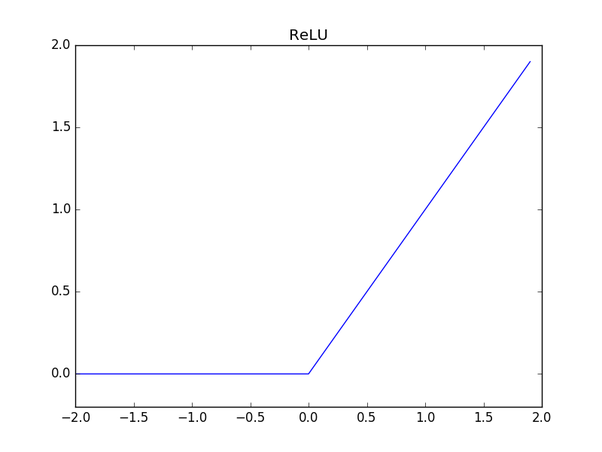
\includegraphics{literature/images/relu.png}
    }
    \caption[Rectified linear units(RELU)]{Rectified linear units}
    \label{lr_fig:ml_relu}
\end{figure}
%
Although it is not differentiable at $z=0$, the gradient descent still acts as expected in practice.
This is because a numerical method rarely finds the local minimal, but ends up with a point that is close enough to the local minimal.
Based on the assumption that a strict zero gradient is not expected, undefined derivatives can be allowed on hidden units.

\paragraph{}
One of the most outstanding advantage of the RELU is that it is extremely easy to optimize.
It is a linear unit expected for the fact that half of its domain yields zero.
As a consequence, the derivative of an RELU is significant if the unit is active.
RELU is applied on top of the existing affine transformation:
\begin{equation}
    \mathbf{h} = g( \mathbf{W}^T \mathbf{x} + \mathbf{b})
\end{equation}
%
Initial values for the transformation matrix are suggested to set with a small positive value as they can make most of the RELU active and let the derivatives pass through.
Because the output remains constant when it is inactive, the unit can not learn anything when it is not active.
Improvements have been proposed recently.
Absolute value rectification that maps $g(z)$ to $|z|$ has been used in object recognition \citep{jarret2009}.
Leaky RELU that gives a small positive value for the derivatives \citep{maas2013} while parametric RELU regards this derivatives as a learnable parameter \citep{He2015}.
Maxout unit \citep{Goodfellow2013} is a further generalization of the RELU.
The maxout unit divides $z$ into groups of $k$ values instead of applying an element-wise function $g(z)$.
The maximum value of the output of all units will be used to represent this group:
\begin{equation}
    g(z)_i = \max_{j\in G^{(i)}} z_j
\end{equation}
%
where $G^{(i)}$ is the set of indices into the input for group $i, \{(i-1)k+1, \dots, ik \}$.
This provides a way of learning a piecewise linear function that responds to multiple directions in the input $x$ space.
It can be regarded as learning the activation function as it actually learn a piecewise linear function.
High fidelity and any convex function can be achieved by maxout unit if a large $k$ is used.
In practice, maxout unit with $k=2$ usually has the same performance compared to the traditional RELU, parametric RELU and Leaky RELU.
Since every maxout unit needs to learn its own parameter, the size of the training set must be large enough to support the learning algorithms, or keep the $k$ value low \citep{Cai2013}.

% \subsection{Back-propagation algorithm}




% ----------------------------------------------------------------- %

\subsection{Performance indicators}
\label{lr_ml:indicators}
\subsubsection{Confusion matrix}
\paragraph{}
A confusion matrix is a matrix used to illustrate the outcome of a classification model on a set of test data whose actual results are known.
    % Please add the following required packages to your document preamble:
    % \usepackage{multirow}
    \begin{table}[]
        \centering
        \caption{Confusion matrix}
        \label{my-label}
        \begin{tabular}{ccccc}
                                & & \multicolumn{2}{c}{\textbf{Predicted}}                 &  \\ \cline{3-4}
                                \multirow{3}{*}[-0.7em]{\textbf{Actual}} &
                                & \multicolumn{1}{|c|}{Refined}        & \multicolumn{1}{c|}{Not refined}    &  \\ \cline{2-4}        
                                & \multicolumn{1}{|c}{Refined}     & \multicolumn{1}{|c|}{True Positive(TP)}  & \multicolumn{1}{c|}{False Negative(FN)} &  \\ \cline{2-4}
                                & \multicolumn{1}{|c}{Not refined} & \multicolumn{1}{|c|}{False Positive(FP)} & \multicolumn{1}{c|}{True Negative(TN)}  &  \\ \cline{2-4}
        \end{tabular}
    \end{table}
%
\subsubsection{Accuracy}
\paragraph{}
Accuracy may be the most intuitive indicator.
It is simply defined as $\frac{TP+TN}{TP+TN+FP+FN}$.
The importance of the accuracy is dependent on the prior since the model can be highly influenced by the prior probability distribution.
For example, a spam detection model is trained from a data set which contains only 10\% of the spam e-mails.
As a consequence, if the model is extremely conservative and classify almost all incoming e-mails as non-spam, it can easily achieve an accuracy of more than 90\% in cross validation which is higher than lots of spam detectors.

\subsubsection{Precision(P)}
\paragraph{}
$$P=TP/(TP+FP)$$
Precision describes the chance that the model gives `true' and it is actually `true'.
In the spam detector example, a high precision can be expected as a conservative model tends to give non-spam unless it has strong confidence.

\subsubsection{Recall rate(R)}
\paragraph{}
$$R=TP/(TP+FN)$$
Recall rate describes the ratio the model gives `true' to the total number of `true's.
In the spam detector example, a low recall rate is expected.

\subsubsection{F1 score}
\paragraph{}
$$F1 = 2*P*R/(P+R)$$
F1 score is an indicator that considers both the precision rate and the recall rate.
It is defined as the harmonic mean of them.

\subsubsection{Receiver operating characteristic(ROC)}
\paragraph{}
ROC is a True Positive Rate(TPR) vs False Positive Rate(FPR) curve (Fig.~\ref{lr_fig:performance_roc}) where $TPR=R$ and $FPR=FP/(FP+TN)$
\begin{figure}[h!]
    \centering
    \scalebox{0.5}{
        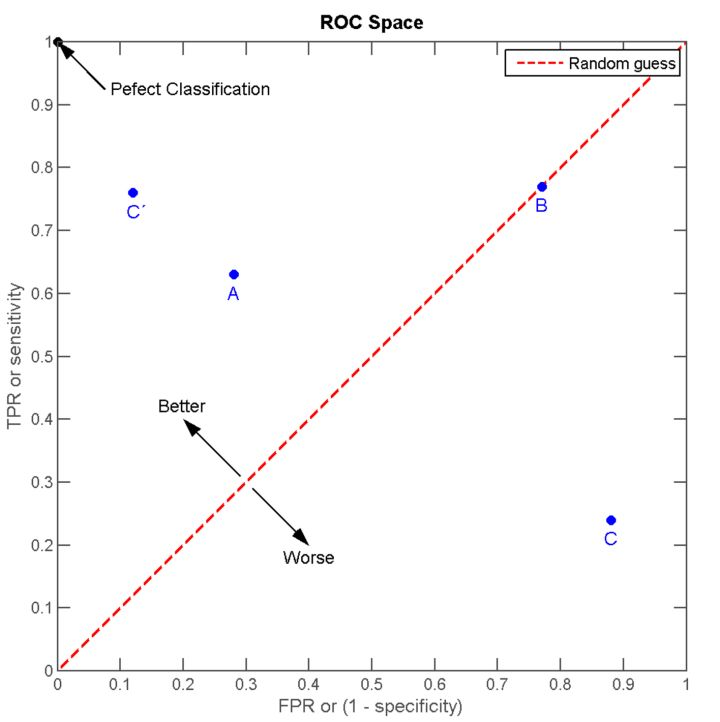
\includegraphics{adaptivity/images/svm_roc.jpg}
    }
    \caption[Receiver operating characteristic(ROC)]{Receiver operating characteristic(ROC)}
    \label{lr_fig:performance_roc}
\end{figure}
%
\subsubsection{Area under the curve(AUC)}
\paragraph{}
As can be seen from the ROC, the larger the area under the curve, the better the classifier is.
Consequently, area under the curve (AUC) becomes another important indicator in machine learning.